\section{Sprint 4}\label{sprint4}
Nach dem dritten von sechs Sprints sind die Grundfunktionen des DlmsQuickAccess implementiert.
In diesem Sprint begann die zweite Hälfte des Projekts und die Arbeit am ersten Zusatzfeature.


\subsection{Favoriten}

\subsubsection{Ziel}
In der Vorbereitungsphase wurde eine Umfrage bei den zukünftigen Nutzern des DlmsQuickAccess durchgeführt.
Wie in Abschnitt \ref{survey} erklärt priorisierten sie dabei mögliche Zusatzfeatures.
Die Funktion, bestimmte Objekte, Attribute oder Methoden als Favoriten markieren und so vereinfacht abrufen zu können erhielt von den Nutzern die höchste Priorität.
Zun den Akzeptanzkriterien der Story gehören folgende Punkte:
\begin{itemize}
   \item Der Benutzer kann Objekte, Attribute und Methoden zu den Favoritenlisten hinzufügen und wider entfernen.
   \item Favorisierte Attribute und Methoden sollen in einer gemeinsam Liste, Objekte in einer eigenen, dargestellt werden.
   \item Neue Einträge sollen jeweils am Ende der Liste erscheinen.
   \item Favorisierte Attribute und Methoden des selben Objekts sollen gruppiert dargestellt werden. Ihre Reihenfolge soll jener innerhalb des Objekts entsprechen.
   \item Die Favoriten sollen Sitzungs- und Produktübergreifend gespeichert werden.
\end{itemize}


\subsubsection{Vorgehen und Schwierigkeiten}
Damit die Favoriten  Sitzungs- und Produktübergreifend bestehen bleiben, muss eine eindeutige Identifikation der favorisierten Objekte persistiert werden.
Als Identifikation bietet sich der Obis Code des Objektes an.
Dieser ist standartisiert und ändert sich von Produkt zu Produkt nicht.
Bei Attributen und Methoden kann der Obis Code in Kombination mit dem Index des Attributes rsp. der Methode für die Identifikation verwendet werden.
Die Obis Codes und Indizes werden dann im \textit{AppicationDataContainer}\footnote{https://docs.microsoft.com/en-us/uwp/api/windows.storage.applicationdatacontainer} gespeichert.
Dabei handelt es sich um einen Key-Value-Store.
Da dieser vom Betriebssystem verwaltet wird, müssen sich bei der Entwicklung keinerlei Gedanken über Dinge wie Files oder Schreibzugriff gemacht werden müsse.

Damit der Benutzer Steuern kann, welche Element zu seinen Favoriten gehören, wurden Objekte, Attribute und Methoden in der Benutzerschnittstelle um das \textit{CanBeFavoriteControl} erweitert.
Dieses besteht aus einem Knopf, mit welchem ein Element favorisiert oder entfavorisiert werden kann.
Das Icon des Knopfs gibt Auskunft darüber, ob das Element bereits Favorit ist oder nicht.
In Abbildung \ref{fig:objectModelWithFavorites} ist das \textit{CanBeFavoriteControl} auf der rechten Seite der Objekte zu sehen.
Das erste Objekt ist nicht favorisiert, das zweite schon.

\begin{figure}
   \centering
   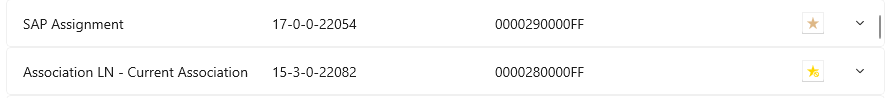
\includegraphics[width=1.0\textwidth]{gfx/objectModelWithFavorites.png}
   \caption{
      Ausschnitt aus DlmsQuickAccess: Ein Objekt ist favorisiert, das andere nicht.
      }
   \label{fig:objectModelWithFavorites}
\end{figure}

Ein Konzept, um die favorisierten Elemente darzustellen ist im Abschnitt \ref{uifavorites} beschrieben.
Dieses wurde im Rahmen dieser Story umgesetzt.
Ursprünglich war geplant, dass lediglich die Namen der favorisierten Objekte aufgelistet werden sollen.
Werden diese angeklickt, so soll das entsprechende Objekt im bereits bestehenden Object Model angezeigt und fokussiert werden.
Dies liess sich so jedoch technisch nicht umsetzten.
Um in der Liste ein bestimmtes Element fokussieren zu können, wir eine Referenz auf dieses benötigt.
Die Instanzen der Controls werden jedoch nicht im C\# Code der Anwendung erstellt, sonder deklarativ mittels XAML.
Deshalb war es nicht möglich, an eine Referenz des gewünschten Controls zu gelangen.

So musste die Idee mit dem Fokussieren verworfen werden.
Stattdessen werden die ganzen Objekte, inklusive Attribute und Methoden, in der Liste der Favoriten dargestellt.
In Abbildung \ref{fig:favoritesUi} ist Liste der favorisierten Objekte gezeigt.
Für die Objekte werden die gleichen Controls wie im Object Model verwendet.
So können die Objekte ebenfalls ein- und ausgeklappt werden.
In der Abbildung ist dies am Beispiel des Objekts \textit{Password Supervision} zu sehen.

\begin{figure}
   \centering
   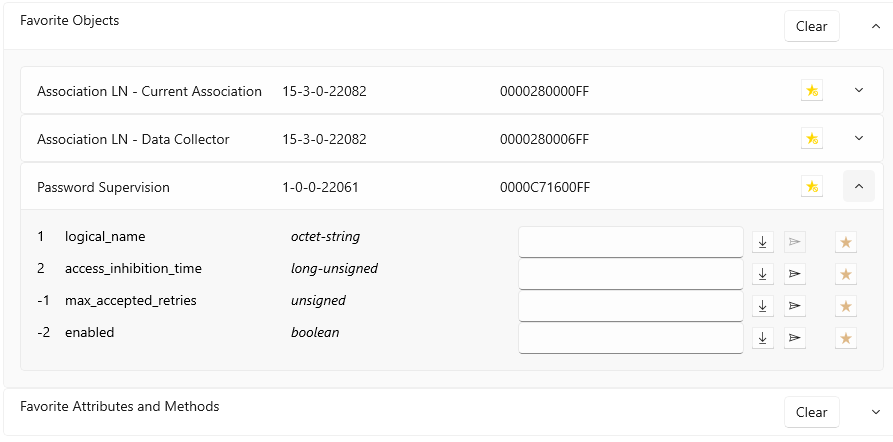
\includegraphics[width=1.0\textwidth]{gfx/favoritesUi.png}
   \caption{
      Die Liste der favorisierten Objekte mit bestehend aus einem Objekt
      }
   \label{fig:favoritesUi}
\end{figure}

Werden einzelne Attribute oder Methoden favorisiert, so erscheinen sie in der Komponente \textit{Favorite Attributes and Methods}, welche in Abbildung \ref{fig:favoriteAttribtuesAndMethods} gezeigt wird.
Die Attribute und Methoden werden jeweils unterhalb des Names des Objektes zu dem sie gehören, angezeigt.
Dies ermöglicht es, dass mit ausgewählten Attribute oder Methoden unterschiedlichster Objekte gearbeitet werden kann, ohne dass hin und her gescrollt werden muss.
\begin{figure}
   \centering
   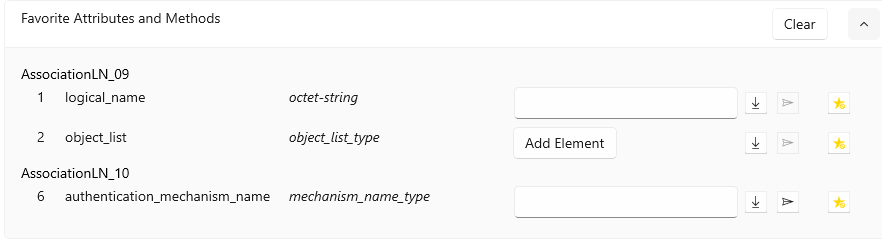
\includegraphics[width=1.0\textwidth]{gfx/favoriteAttributeAndMethods.png}
   \caption{
     Auflistung der favorisierten Attribute und Methoden
      }
   \label{fig:favoriteAttribtuesAndMethods}
\end{figure}

Die Views des Object Model und jener der Favoritenliste nutzen die selben ViewModel Instanzen.
Wird bei einem Element aus der Favoritenliste ein Lesebefehl ausgeführt, so wird der gelesene Wert auch im Object Model angezeigt.